\documentclass[6pt,a4paper]{article}
\usepackage{../ve230}
\usetikzlibrary{positioning}

\begin{document}


\subsection{2-11}
\begin{center}
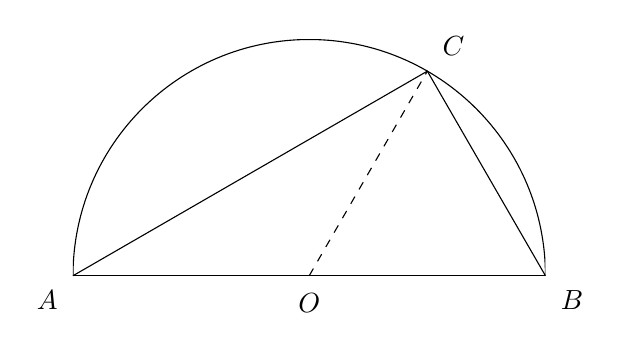
\begin{tikzpicture}[baseline=(current bounding box.north),scale=2]
\begin{scope}
    \clip (-1.5,0) rectangle (1.5,1.5);
    \draw (0,0) circle(1.5);
    \draw (-1.5,0) -- (1.5,0);
\end{scope}
\node[below left= 1mm of {(-1.5,0)}] {$A$};
\node[below= 1mm of {(0,0)}] {$O$};
\node[below right= 1mm of {(1.5,0)}] {$B$};
\node[above right= 1mm of {(60:1.5)}] {$C$};
\draw (-1.5,0) -- (60:1.5) -- (1.5,0);
\draw[dashed] (0,0) -- (60:1.5);
\end{tikzpicture}
\end{center}

Since $OA=OB=OC$, we know $\angle OAC=\angle OCA$ and $\angle OBC=\angle OCB$. And since $ABC$ is an triangle, $\angle OAC+\angle OBC+\angle ACB=\pi$, we can simply find that $\angle ACB=\pi/2$, so that an angle inscribed in a semicircle is a right angle.

\subsection{2-17}
\begin{enumerate}[label=\alph*)]
\item 
$$|\mathbf{E}|=|\mathbf{a_R}(25/R^2)|=|\mathbf{a_R}|\cdot\frac{25}{3^2+4^2+5^2}=\frac{1}{2}.$$
$$E_x=|\mathbf{E}|\cdot\frac{x}{R}=\frac{1}{2}\cdot\frac{-3}{\sqrt{3^2+4^2+5^2}}=-\frac{3\sqrt{2}}{20}.$$
\item
$$\cos\theta=\frac{\mathbf{E}\cdot\mathbf{B}}{|\mathbf{E}||\mathbf{B}|}=\frac{-3\cdot2+4\cdot-2-5\cdot1}{\sqrt{3^2+4^2+5^2}\cdot\sqrt{2^2+2^2+1^1}}=-\frac{19\sqrt{2}}{30},$$
$$\theta=\arccos-\frac{19\sqrt{2}}{30}\approx \SI{2.681}{\radian}.$$
\end{enumerate}

\subsection{2-21}
$$\int_{P_1}^{P_2}\mathbf{E}\cdot d\mathbf{l}=\int_{P_1}^{P_2}(\mathbf{a_x}y+\mathbf{a_y}x)(\mathbf{a_x}dx+\mathbf{a_y}dy)=\int_{P_1}^{P_2}(ydx+xdy)$$
\begin{enumerate}[label=\alph*)]
\item
$$\int_{P_1}^{P_2}\mathbf{E}\cdot d\mathbf{l}=\int_{P_1}^{P_2}(y\cdot4ydy+2y^2\cdot dy)=\int_1^2 6y^2dy=14.$$
\item
$$x=6y-4,$$
$$\int_{P_1}^{P_2}\mathbf{E}\cdot d\mathbf{l}=\int_{P_1}^{P_2}[y\cdot6dy+(6y-4)\cdot dy]=\int_1^2 (12y-4)dy=14.$$
\end{enumerate}

\subsection{2-26}
\begin{enumerate}[label=\alph*)]
\item
$$\nabla\cdot f_1(\mathbf{R})=\frac{1}{R^2}\cdot\frac{\partial}{\partial R}(R^n\cdot R^2)=(n+2)R^{n-1}.$$
\item
$$\nabla\cdot f_2(\mathbf{R})=\frac{1}{R^2}\cdot\frac{\partial}{\partial R}(k/R^2\cdot R^2)=0.$$
\end{enumerate}

\subsection{2-29}
$$\nabla\cdot\mathbf{A}=\frac{1}{r}\cdot\frac{\partial}{\partial r}(r^2\cdot r)+\frac{\partial}{\partial z}(2z)=3r+2.$$
$$\int_V\nabla\cdot\mathbf{A}dV=\int_V(3r+2)dV=\int_0^4\int_0^{2\pi}\int_0^5(3r+2)rdrd\theta dz=1200\pi.$$
$$\oint_S\mathbf{A}dS=\int_0^4\int_0^{2\pi}(\mathbf{a_r}r^2)rd\theta dz\mathbf{a_r}+\int_0^{2\pi}\int_0^52z\mathbf{a_z}rdrd\theta\mathbf{a_z}=1000\pi+200\pi=1200\pi.$$
So $$\int_V\nabla\cdot\mathbf{A}dV=\oint_S\mathbf{A}dS.$$

\subsection{2-33}
$$\nabla\cdot(\mathbf{E}\times\mathbf{H})=\frac{\partial}{\partial x}(E_yH_z-E_zH_y)+\frac{\partial}{\partial y}(E_zH_x-E_xH_z)+\frac{\partial}{\partial z}(E_xH_y-E_yH_x),$$
$$\mathbf{H}\cdot(\nabla\times\mathbf{E})=H_x\left(\frac{\partial E_z}{\partial y}-\frac{\partial E_y}{\partial z}\right)+H_y\left(\frac{\partial E_x}{\partial z}-\frac{\partial E_z}{\partial x}\right)+H_z\left(\frac{\partial E_y}{\partial x}-\frac{\partial E_x}{\partial y}\right),$$
$$\mathbf{E}\cdot(\nabla\times\mathbf{H})=E_x\left(\frac{\partial H_z}{\partial y}-\frac{\partial H_y}{\partial z}\right)+E_y\left(\frac{\partial H_x}{\partial z}-\frac{\partial H_z}{\partial x}\right)+E_z\left(\frac{\partial H_y}{\partial x}-\frac{\partial H_x}{\partial y}\right).$$
Since
$$\frac{\partial}{\partial x}AB=A\frac{\partial B}{\partial x}+B\frac{\partial A}{\partial x},$$
we can find that
$$\nabla\cdot(\mathbf{E}\times\mathbf{H})=\mathbf{H}\cdot(\nabla\times\mathbf{E})-\mathbf{E}\cdot(\nabla\times\mathbf{H}).$$

\subsection{2-35}
$$\Delta s_u=R^2\sin\theta\Delta\theta\Delta\phi,$$
\begin{align*}
\oint_{C_u}\mathbf{A}\cdot d\mathbf{l}=&A_\theta\cdot(R,\theta,\phi-\Delta\phi/2)R\Delta\theta-A_\theta\cdot(R,\theta,\phi+\Delta\phi/2)R\Delta\theta+\\
&A_\phi\cdot(R,\theta+\Delta\theta/2,\phi)R\Delta\phi\sin(\theta+\Delta\theta/2)-A_\phi\cdot(R,\theta-\Delta\theta/2,\phi)R\Delta\phi\sin(\theta-\Delta\theta/2)\\
=&-\frac{\partial A_\theta}{\partial\phi}R\Delta\phi\Delta\theta+\frac{\partial A_\phi\sin\theta}{\partial\theta}R\Delta\phi\Delta\theta.
\end{align*}
\begin{align*}
(\nabla\times\mathbf{A})_u&=\lim_{\Delta s_u\to0}\frac{1}{\Delta s_u}\oint_{C_u}\mathbf{A}\cdot d\mathbf{l}=\lim_{\Delta s_u\to0}\frac{1}{R^2\sin\theta\Delta\theta\Delta\phi}\cdot\left(-\frac{\partial A_\theta}{\partial\phi}+\frac{\partial A_\phi\sin\theta}{\partial\theta}\right)R\Delta\phi\Delta\theta\\
&=\frac{1}{R\sin\theta}\cdot\left(-\frac{\partial A_\theta}{\partial\phi}+\frac{\partial A_\phi\sin\theta}{\partial\theta}\right).
\end{align*}
$$$$

\subsection{2-39}
\begin{enumerate}[label=\alph*)]
\item
$$\nabla\times\mathbf{F}=\mathbf{a_x}(c_3+3)+\mathbf{a_y}(c_1-1)+\mathbf{a_z}c_2=\mathbf{0},$$
$$c_1=1,c_2=0,c_3=-3.$$
\item
$$\nabla\cdot\mathbf{F}=1+0+c_4=0,$$
$$c_4=-1.$$
\item
$$\mathbf{F}=-\nabla V=\mathbf{a_x}(x+z)+\mathbf{a_y}(-3z)+\mathbf{a_z}(x-3y-z),$$
$$V=-\frac{1}{2}x^2-xz+3yz+\frac{1}{2}z^2+C.$$
\end{enumerate}


\subsection{3-8}
\begin{center}
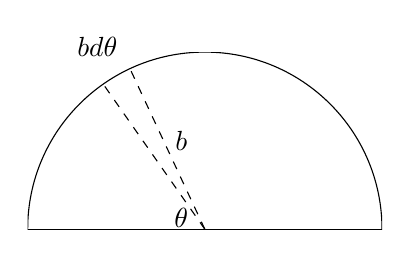
\begin{tikzpicture}[baseline=(current bounding box.north),scale=1.5]
\begin{scope}
    \clip (-1.5,0) rectangle (1.5,1.5);
    \draw (0,0) circle(1.5);
    \draw (-1.5,0) -- (1.5,0);
\end{scope}
\node[above left=0.5mm of {(115:1.5)}] {$bd\theta$};
\node at (-0.2,0.75) {$b$};
\node at (-0.2,0.1) {$\theta$};
\draw[dashed] (0,0) -- (115:1.5);
\draw[dashed] (0,0) -- (125:1.5);
\end{tikzpicture}
\end{center}

$$dQ=bd\theta\rho_l,$$
$$dE=\frac{dQ}{4\pi\epsilon_0b^2}=\frac{\rho_l}{4\pi\epsilon_0b}d\theta,$$
$$|\mathbf{E}|=\int_0^\pi dE\sin\theta=\frac{\rho_l}{4\pi\epsilon_0b}\int_0^\pi\sin\theta d\theta=\frac{\rho_l}{2\pi\varepsilon_0b}.$$
The direction is downwards.

\subsection{3-9}
\begin{center}
\begin{tikzpicture}[baseline=(current bounding box.north),scale=1.5]
\begin{scope}
    \clip (-2,-2) rectangle (2,2);
    \draw (-1.732,-1) -- (1.732,-1) -- (0,1.732) -- (-1.732,-1);
\end{scope}
\node[above left=1mm of {(-0.866,0.366)}] {$\rho_{l2}$};
\node[below=1mm of {(0,-1)}] {$-\rho_{l1}$};
\node[above right=1mm of {(0.866,0.366)}] {$\rho_{l3}$};
\end{tikzpicture}
\end{center}

$$dQ=\rho dl,$$
$$dE=\frac{dQ}{4\pi\varepsilon_0(l^2+L^2/12)}=\frac{\rho}{4\pi\varepsilon_0}\cdot\frac{dl}{l^2+L^2/12},$$
$$|\mathbf{E_1}|=\int_{-L/2}^{L/2}dE\cdot\sqrt{\frac{L^2/12}{l^2+L^2/12}}=\frac{3\rho_{l1}}{2\pi\varepsilon_0 L},$$
$$|\mathbf{E_2}|=|\mathbf{E_3}|=\frac{1}{2}|\mathbf{E_1}|=\frac{3\rho_{l1}}{4\pi\varepsilon_0 L}.$$
$$|\mathbf{E}|=|\mathbf{E_1}|-\frac{1}{2}|\mathbf{E_2}|-\frac{1}{2}|\mathbf{E_3}|=\frac{3\rho_{l1}}{4\pi\varepsilon_0 L}.$$
The direction is upwards.

\subsection{3-12}
\begin{enumerate}[label=\alph*)]
\item 
For $0<r<a$, $\mathbf{E}=\mathbf{0}$.

For $a<r<b$, $$2\pi aL\cdot\frac{\rho_{sa}}{\varepsilon_0}=2\pi rL\cdot E,$$
$$\mathbf{E}=\frac{a\rho_{sa}}{\varepsilon_0 r}\mathbf{a_r}.$$

For $b<r$, $$2\pi aL\cdot\frac{\rho_{sa}}{\varepsilon_0}+2\pi bL\cdot\frac{\rho_{sb}}{\varepsilon_0}=2\pi rL\cdot E,$$
$$\mathbf{E}=\frac{a\rho_{sa}+b\rho_{sb}}{\varepsilon_0 r}\mathbf{a_r}.$$
\item
$$\frac{a\rho_{sa}+b\rho_{sb}}{\varepsilon_0 r}=0,$$
$$a=-\frac{\rho_{sb}}{\rho_{sa}}b.$$
\end{enumerate}

\subsection{3-13}
$$W=-\int\mathbf{E}qd\mathbf{l}=2\mu \int(\mathbf{a_x}y+\mathbf{a_y}x)(\mathbf{a_x}dx+\mathbf{a_y}dy)=2\mu \int ydx+xdy.$$
\begin{enumerate}[label=\alph*)]
\item 
$$W=2\mu \int ydx+xdy=2\mu C\int_2^8 4y^2dy+2y^2dy=28\mu.$$
\item 
$$x=6y-4,$$
$$W=2\mu \int ydx+xdy=2\mu C\int_2^8 6ydy+(6y-4)dy=28\mu.$$
\end{enumerate}

\subsection{3-16}
\begin{enumerate}[label=\alph*)]
\item 
$$dQ=\rho_l dl,$$
$$dV=\frac{dQ}{4\pi\varepsilon_0\sqrt{l^2+y^2}}=\frac{\rho_l}{4\pi\varepsilon_0}\cdot\frac{dl}{\sqrt{l^2+y^2}},$$
$$V=\int_{-L/2}^{L/2}dV=\frac{\rho_l}{4\pi\varepsilon_0}\int_{-L/2}^{L/2}\frac{1}{\sqrt{l^2+y^2}} dl=\frac{\rho_l}{2\pi\varepsilon_0}{\rm arcsinh}\frac{L}{2y}.$$
\item
$$dE=\frac{dQ}{4\pi\varepsilon_0(l^2+y^2)}=\frac{\rho_l}{4\pi\varepsilon_0}\cdot\frac{dl}{l^2+y^2},$$
$$\mathbf{E}=\mathbf{a_y}\int_{-L/2}^{L/2}dE\cdot\sqrt{\frac{y^2}{l^2+y^2}}=\frac{\rho_l}{2\pi\varepsilon_0}\cdot\frac{y}{\sqrt{L^2+4y^2}}\mathbf{a_y}.$$
\item
$$-\nabla V=-\frac{dV}{dy}\mathbf{a_y}=\frac{\rho_l}{4\pi\varepsilon_0}\cdot\frac{L}{\sqrt{L^2+4y^2}}\mathbf{a_y}=\mathbf{E}.$$
\end{enumerate}

\subsection{3-19}
$$dQ=\frac{Q}{h} dz,$$
$$dV=\frac{dQ}{4\pi\varepsilon_0\sqrt{b^2+z^2}}=\frac{Q}{4\pi\varepsilon_0h\sqrt{b^2+z^2}}dz.$$
\begin{enumerate}[label=\alph*)]
\item 
$$V=\int_{z-h}^zdV=\frac{Q}{4\pi\varepsilon_0h}\int_{z-h}^z\frac{1}{\sqrt{b^2+z^2}}dz=\frac{Q}{4\pi\varepsilon_0h}\left[{\rm arcsinh}\frac{z}{b}-{\rm arcsinh}\frac{z-h}{b}\right].$$
$$\mathbf{E}=-\nabla V=-\frac{dV}{dz}\mathbf{a_z}=-\frac{Q}{4\pi\varepsilon_0h}\left[\frac{1}{\sqrt{b^2+z^2}}-\frac{1}{\sqrt{b^2+(z-h)^2}}\right]\mathbf{a_z}.$$
\item
$$V=\int_0^zdV+\int_0^{h-z}dV=\frac{Q}{4\pi\varepsilon_0h}\left[{\rm arcsinh}\frac{z}{b}+{\rm arcsinh}\frac{h-z}{b}\right].$$
$$\mathbf{E}=-\nabla V=-\frac{dV}{dz}\mathbf{a_z}=-\frac{Q}{4\pi\varepsilon_0h}\left[\frac{1}{\sqrt{b^2+z^2}}-\frac{1}{\sqrt{b^2+(h-z)^2}}\right]\mathbf{a_z}.$$
\end{enumerate}

\subsection{3-22}
\begin{enumerate}[label=\alph*)]
\item 
$$\rho_{ps}=\mathbf{P}\cdot\mathbf{a_n}|_{n=L/2}=\frac{1}{2}P_0L.$$
$$\rho_p=-\nabla\cdot\mathbf{P}=-3P_0.$$
\item
$$Q_s=\oint_S\rho_{ps}dS=\frac{1}{2}P_0L\cdot 6L^2=3P_0L^3,$$
$$Q_v=\int_v\rho_pdV=\int_{-L/2}^{L/2}\int_{-L/2}^{L/2}\int_{-L/2}^{L/2}\rho_pdzdydx=-3P_0L^3,$$
$$Q=Q_s+Q_v=0.$$
\end{enumerate}

\subsection{3-23}
Let $\mathbf{P}=\mathbf{a_p}P_0$, $\theta=\langle \mathbf{P},\mathbf{a_n} \rangle$,
$$\rho_{ps}(\theta)=\mathbf{P}\cdot\mathbf{a_n}=P_0\cos\theta,$$
$$dE_\theta=dv\cdot\frac{\rho_{ps}}{4\pi\varepsilon_0R^2}\cdot\cos\theta=2\pi R^2\sin\theta d\theta\cdot\frac{P_0\cos\theta}{4\pi\varepsilon_0R^2}\cdot\cos\theta=\frac{P_0\sin\theta\cos\theta^2}{2\varepsilon_0}d\theta.$$
$$|\mathbf{E}|=\int dE_\theta=\int_0^\pi\frac{P_0\sin\theta\cos\theta^2}{2\varepsilon_0}d\theta=\frac{P_0}{3\varepsilon_0},$$
$$\mathbf{E}=\mathbf{a_p}\frac{P_0}{3\varepsilon_0}=\frac{\mathbf{P}}{3\varepsilon_0}.$$

\subsection{3-25}
$$E_{2t}=E_{1t}=\mathbf{a_x}2y-\mathbf{a_y}3x.$$
Since $\rho_s=0$,
$$\varepsilon_{r1}E_{1n}=\varepsilon_{r2}E_{2n},$$
$$E_{2n}=\frac{\varepsilon_{r1}}{\varepsilon_{r2}}E_{1n}=\frac{2}{3}\cdot\mathbf{a_z}5=\mathbf{a_z}\frac{10}{3}.$$
$$E_2=E_{2t}+E_{2n}=\mathbf{a_x}2y-\mathbf{a_y}3x+\mathbf{a_z}\frac{10}{3}.$$
$$\mathbf{D_2}=\varepsilon_2\mathbf{E_2}=3\varepsilon_0\left(\mathbf{a_x}2y-\mathbf{a_y}3x+\mathbf{a_z}\frac{10}{3}\right).$$

\subsection{3-28}
Obviously, $\mathbf{E_3}$ is parallel to $\mathbf{E_2}$, so we only need to find $\varepsilon_{r2}$ so that $\mathbf{E_2}$ is parallel to  the x-axis.
$$E_{1t}=E_{2t}=-3.$$
$$\varepsilon_{r1}E_{1n}=\varepsilon_{r2}E_{2n},$$
$$E_{2n}=\frac{\varepsilon_{r1}}{\varepsilon_{r2}}E_{1n}=\frac{1}{\varepsilon_{r2}}\cdot5=\frac{5}{\varepsilon_{r2}}.$$
$$E_{2t}\cos\theta+E_{2n}\cos\theta=0,$$
$$-3+\frac{5}{\varepsilon_{r2}}=0,$$
$$\varepsilon_{r2}=\frac{5}{3}.$$

\subsection{3-32}
$$C_1=\frac{2\pi\varepsilon L}{\ln\frac{b}{r_i}}=\frac{2\pi\varepsilon_0\varepsilon_{r_1}L}{\ln\frac{b}{r_i}},$$
$$C_2=\frac{2\pi\varepsilon L}{\ln\frac{r_o}{b}}=\frac{2\pi\varepsilon_0\varepsilon_{r_2}L}{\ln\frac{r_o}{b}},$$
$$C=\frac{1}{\frac{1}{C_1}+\frac{1}{C_2}}=\frac{2\pi\varepsilon_0L}{\frac{1}{\varepsilon_{r_1}}\ln\frac{b}{r_i}+\frac{1}{\varepsilon_{r_3}}\ln\frac{r_o	}{b}},$$
$$\frac{C}{L}=\frac{2\pi\varepsilon_0}{\frac{1}{\varepsilon_{r_1}}\ln\frac{b}{r_i}+\frac{1}{\varepsilon_{r_3}}\ln\frac{r_o}{b}}.$$

\subsection{3-43}
$$dW_e=Vdq=\frac{q}{C}dq,$$
$$W_e=\int dW_e=\int_0^Q \frac{q}{C}dq=\frac{Q^2}{2C}.$$
Since $Q=CV$, we can also get
$$W_e=\frac{1}{2}CV^2=\frac{1}{2}QV.$$


\end{document}
